% Copyright 2004 by Till Tantau <tantau@users.sourceforge.net>.
%
% In principle, this file can be redistributed and/or modified under
% the terms of the GNU Public License, version 2.
%
% However, this file is supposed to be a template to be modified
% for your own needs. For this reason, if you use this file as a
% template and not specifically distribute it as part of a another
% package/program, I grant the extra permission to freely copy and
% modify this file as you see fit and even to delete this copyright
% notice. 

\documentclass{beamer}

\usetheme{Madrid}

\title[Sparse Noise]{Finding meaningful cluster structure \\ amidst background noise} % The short title appears at the bottom of every slide, the full title is only on the title page

\author[Shrinu Kushagra]
{%
  \texorpdfstring{
    \begin{columns}%[onlytextwidth]
      \column{.75\linewidth}
      \centering
      \vspace{25pt}\\ Shrinu Kushagra\\ \vspace{15pt}
      Oct 04, 2016 \\ \vspace{15pt}
      Joint work with Samira Samadi and Shai Ben-David
    \end{columns}
    \vspace{5pt}
	  \begin{figure}
	  
\includegraphics[trim = 0 50 0 0, clip, width=0.3\linewidth]{logo.pdf}
	  \end{figure}  
  }
  {}
}


\AtBeginSubsection[]
{
  \begin{frame}<beamer>
  \frametitle{Outline}
    \tableofcontents[currentsection]
  \end{frame}
}

\newcommand{\mc}{\mathcal}

% Let's get started
\begin{document}

\begin{frame}
  \titlepage
\end{frame}

\begin{frame}{Outline}
  \tableofcontents
  % You might wish to add the option [pausesections]
\end{frame}

% Section and subsections will appear in the presentation overview
% and table of contents.
\section{Introduction}

\begin{frame}{What is clustering}
  Input: A list of objects $\mc X$\\
  Output: 
  \begin{itemize}
  \item {
    Clustering is typically an {\color{red}under-specified} task
     \begin{itemize}
         \item Which algorithm/objective to choose?
         \item Sensitive to the choice of metric, etc.         
         \item Solution is not unique
     \end{itemize}
  }
  \pause
  \item {   
    Clustering is {\color{red}computationally expensive}
     \begin{itemize}
         \item Solving K-means, K-median, K-medoids, K-center, Min Normalized-Cut, ... is NP-hard 
     \end{itemize}
  }
  \pause
  \item {What can we do?}
  
  \end{itemize}
\end{frame}


\begin{frame}{Our Approach}
  \begin{itemize}
  \item {
     Learner can {\color{red}interact} with an expert to get ``{\color{red} advice}''
     
  }
  \pause
  \item {   
    Same-Cluster Query
    \begin{itemize}
        \item Do $x_1$ and $x_2$ belong to the same cluster?
        \item No need to know the number of clusters beforehand
    \end{itemize}
  }
  \pause 
  \item {   
    Learner should output the ``true'' clustering
    \begin{itemize}
        \item Consistent with expert's knowledge
    \end{itemize}
  }
  \pause 
  \item Query complexity?
  \item Computational complexity?
  
  \end{itemize}
\end{frame}

\section{Previous Work}

\begin{frame}{Dealing with Computational Complexity}
  \begin{itemize}
  
    \item Hardness of clustering
    \begin{itemize}
        \item 2-means (Dasgupta (2009))
        \item Planar k-means (Mahajan et. al (2009), Vattani (2009))
        \item k-median, k-center, ...
    \end{itemize}
    \pause
    \item Approximate algorithms for K-means
    \begin{itemize}
        \item $(9+\epsilon)$-approximation (Kanungo et al. (2002))
        \item PTAS for fixed $k$ (Kumar et al. (2004))
        \item NP-hard in general (Awasthi et al. (2015))
    \end{itemize}
    
    \pause
    \item Niceness assumptions (Awasthi et al. (2012), Ackerman and Ben-David (2009))
    \begin{itemize}
        \item Avoid worst-case scenarios
        \item From deep learning to SAT solvers
        \item In clustering: clusters are ``well-separated''
        \item Quest for finding realistic and testable notions
    \end{itemize}
    
    \pause
    \item Heuristics
        \begin{itemize}
            \item Loyd algorithm, local search, ...
            \item Relaxation/``Convexification''
        \end{itemize}
        
        
  \end{itemize}
\end{frame}


\begin{frame}{Dealing with Under-Specificity}
  \begin{itemize}
  
    \item Constrained Clustering (Wagstaff et al. (2000))
    \begin{itemize}
        \item ``Must/Cannot'' constraints
        \item Heuristic approach
    \end{itemize}
    
    \pause
    
    \item Metric Learning using Side-Information (Xing et. al (2003), Alipanahi et. al (2008))
        \begin{itemize}
            \item Maps points of the same cluster close to each other and ... 
            \item How can we ``consistently'' cluster the points in the new space?
        \end{itemize}
    \pause
    \item Metric Learning for K-means (Ashtiani and Ben-David (2015))
    \begin{itemize}
        \item Receives the clustering of a small subset of data
        \item Finds a ``consistent'' mapping
        \item Sample complexity analysis only
    \end{itemize}
    \pause
    \item Interactive Clustering (Balcan and Blum (2008))
    \begin{itemize}
        \item Merge-Split model 
        \item Hard to evaluate long queries
    \end{itemize}

  \end{itemize}
\end{frame}



\section{Big Picture}

\begin{frame}{Problem Setting}
  
  %\begin{figure}
  %  \begin{overprint}
  %      \onslide<1> \centering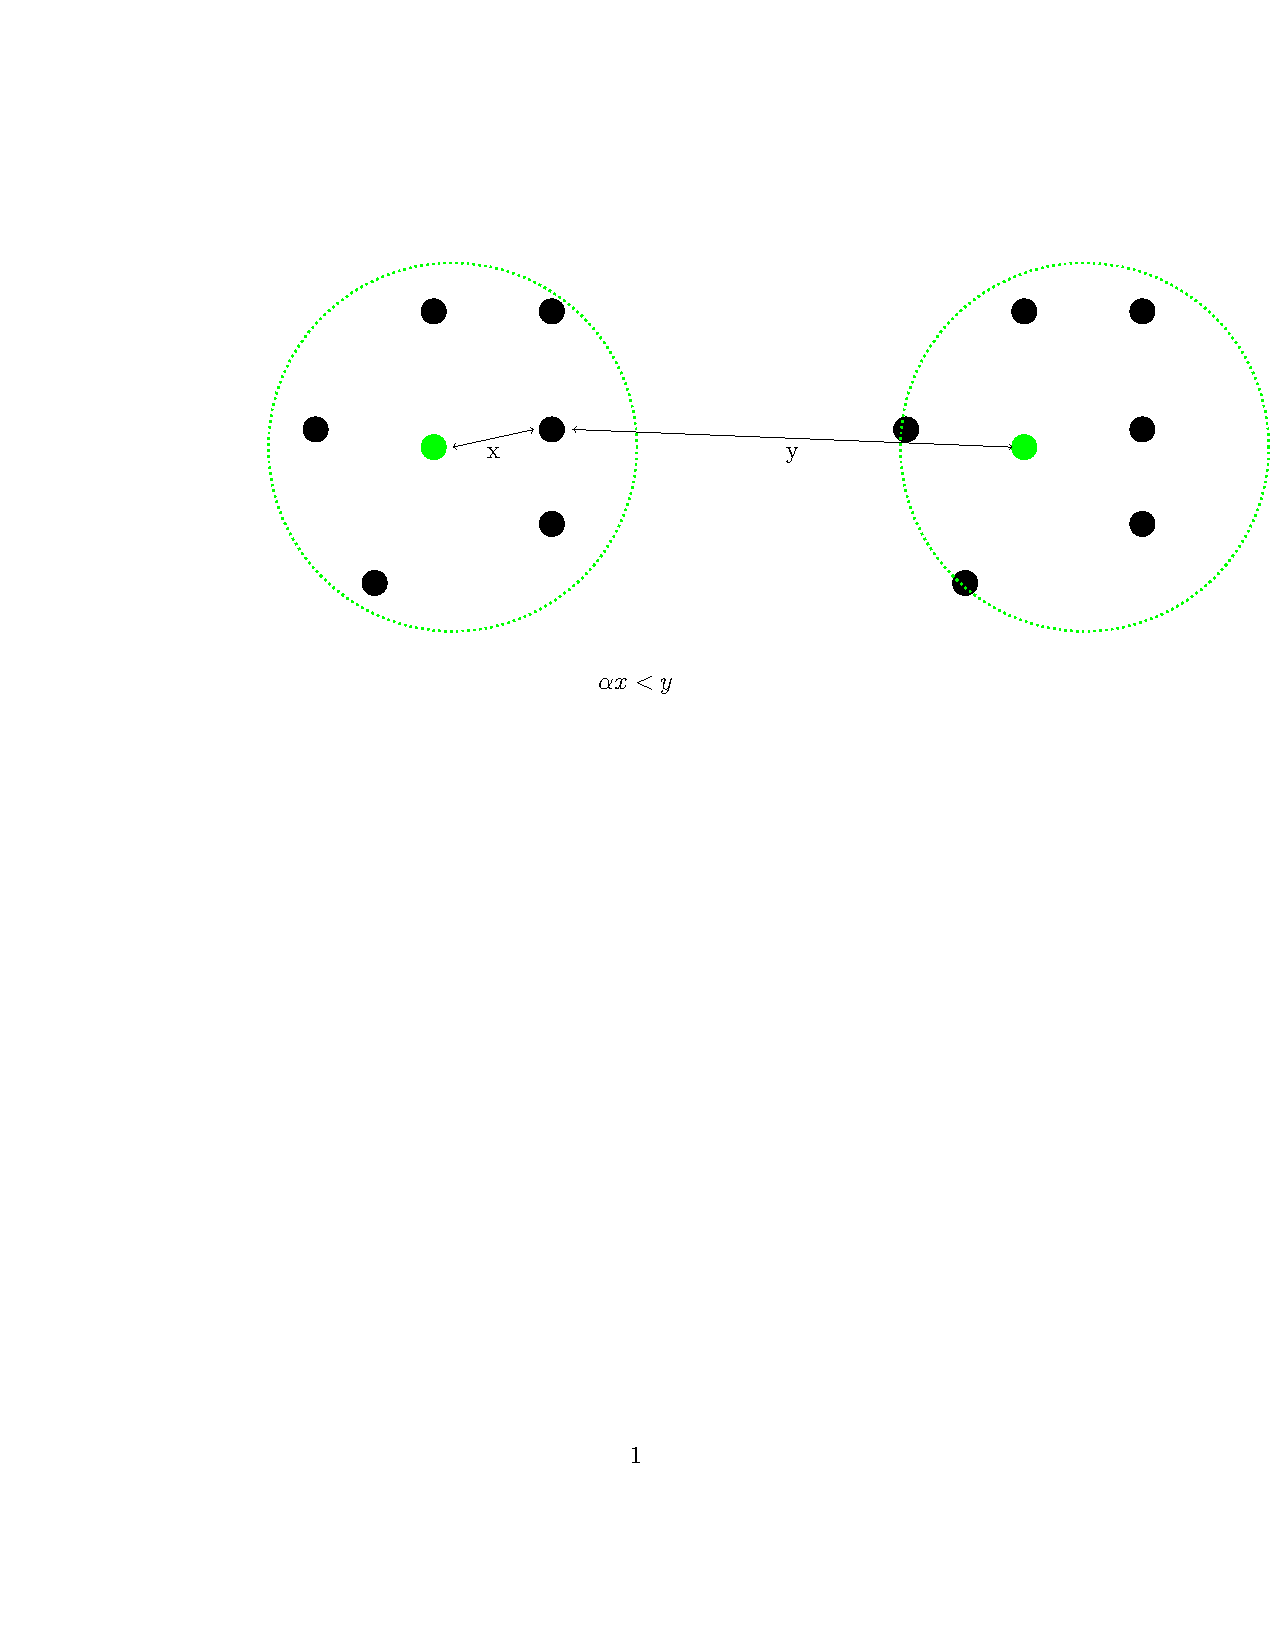
\includegraphics[scale=0.5]{Figures/1.png}
  %  \end{overprint}
  %\end{figure}
    
  \begin{itemize}
    \item $X = \{x_i\}_{i=1}^{n} \subset \mathbb{R}^d$
    \item $k$ is the number of clusters

  \end{itemize}
\end{frame}

\begin{frame}{Well-Clustered Data}
  \begin{itemize}
    
    \item Nicely separated clusters 

  \end{itemize}
\end{frame}


\begin{frame}{$\gamma$-Margin Condition}
  \begin{itemize}
	\item Admits a polynomial time algorithm for $\gamma > 2$
    \item What about smaller $\gamma$, especially $\gamma \rightarrow 0$?
    \item Can we use queries?

  \end{itemize}
\end{frame}



\begin{frame}{Outline of Contributions}
  \begin{itemize}
    
    \item Clustering with same-cluster queries
    
    \begin{itemize}
        \item Polynomial time algorithm (in $k$, $d$, $n$, and $\frac{1}{\gamma}$)
        \item Reasonably small number of queries
        \item Looking for the ``exact'' solution
    \end{itemize}
    
    \pause
    \item The case of K-means clustering
    \begin{itemize}
        \item Oracle conforms to the optimal k-means solution
        \item Hardness result and lower bounds
    \end{itemize}

  \end{itemize}
\end{frame}

\section{Algorithmic Approach}

\begin{frame}{Clustering with Advice}
  \begin{itemize}
    
    \item $\theta(n^2)$ is trivial 
    
    \begin{itemize}
        \item We want at most $O(\log n)$ queries
    \end{itemize}

  \end{itemize}
\end{frame}

\begin{frame}{Active Clustering Algorithm}

    \begin{block}
    


    \begin{itemize}
    

    \item Uniformly select points and find their corresponding cluster
    \item Continue until we have ``enough'' points from one cluster
    \item Estimate the center
    \item Binary search to find the boundary
    \item Remove the cluster
    \item Continue with the remaining clusters
      \end{itemize}
  
  \end{block}
  \pause
  \begin{itemize}
      \item Don't ask the oracle the same query again
      \item Don't need to have $k$ in advance
  \end{itemize}

\end{frame}

\begin{frame}{Analysis}
  \begin{itemize}
    
    \item How many points from each cluster?
    \begin{itemize}
        \item Enough to estimate the center
        \item $\|\mu - \hat{\mu}\| < \frac{\gamma R}{2}$

    \end{itemize}
    \pause
    
    \item Generalized Hoeffding's inequality for Hilbert spaces
    \begin{itemize}
        \item Need $O(\frac{\log \frac{1}{\delta}}{\gamma ^2})$ points from each cluster
        \item Independent of $d$
    \end{itemize}    
    \pause
    \item Number of queries for each cluster
    \begin{itemize}
        \item $O(k\frac{\log \frac{k}{\delta}}{\gamma ^2})$ for finding the center
        \item $\log n$ for binary search
    \end{itemize}        
    \pause
    \begin{theorem}
        The proposed algorithm finds the exact clustering with probability at least $1-\delta$ and
        \begin{itemize}
            \item Asks $O(k \log n  + \frac{k^2 \log \frac{k}{\delta}}{\gamma ^2})$ queries
            \item Runs in $O(kn \log n  + \frac{k^2 \log \frac{k}{\delta}}{\gamma ^2})$ time       
            \end{itemize}   
    \end{theorem}


  \end{itemize}
\end{frame}


\section{The case of K-means Clustering}

\begin{frame}{Lower bound for Number of Queries}
  \begin{itemize}
    
    \item Still hard if learner asks ``a few'' queries?
    \pause
    \item NP-hard with $O(\log n + \log k)$ queries
    \begin{itemize}
        \item Simulation trick
    \end{itemize}
    
  \end{itemize}
\end{frame}



\section{Conclusions}

\begin{frame}{Summary}
  \begin{itemize}
    
    \item Interactive model for clustering
    \pause
    \item A weaker notion of ``clusterability'' 
    \pause
    \item An efficient algorithm for this setting
    \pause
    \item Makes NP-hard problems easy using rather small queries
    \pause

  \end{itemize}
\end{frame}

\begin{frame}{Future Work}
  \begin{itemize}
    
    \item Noisy oracle
    \begin{itemize}
        \item Adversarial?
    \end{itemize}
    \pause
    \item Abstentions
    \begin{itemize}
        \item Possible with $O(\log nk)$ abstentions
    \end{itemize}
    \pause
    \item Other clustering problems?

  \end{itemize}
\end{frame}


\begin{frame}
    \Huge{\centerline{Thank You!}}
\end{frame}

%----------------------------------------
%        Figure Samples
%----------------------------------------

% All of the following is optional and typically not needed. 
\appendix
\section<presentation>*{\appendixname}
\subsection<presentation>*{For Further Reading}

%\begin{frame}[allowframebreaks]
  %\frametitle<presentation>{For Further Reading}
   % 
  %\begin{thebibliography}{10}
    
  %\beamertemplatebookbibitems
  % Start with overview books.

  %\bibitem{Author1990}
   % A.~Author.
    %\newblock {\em Handbook of Everything}.
    %\newblock Some Press, 1990.
 
    
  %\beamertemplatearticlebibitems
  % Followed by interesting articles. Keep the list short. 

  %\bibitem{Someone2000}
   % S.~Someone.
    %\newblock On this and that.
    %\newblock {\em Journal of This and That}, 2(1):50--100,
    %2000.
  %\end{thebibliography}
%\end{frame}

\end{document}


